\chapter{DEPLOYMENT}
 
\section{Welcome form:}
 \begin{figure}[H]
\centering
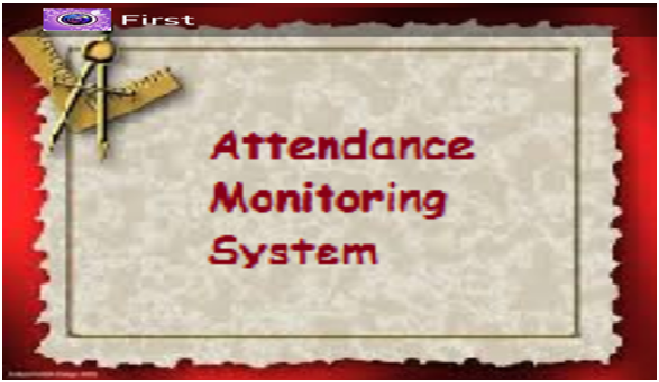
\includegraphics[width=5in]
{AA1}
\caption{Welcome Form}
\end{figure}

This is the first form of our application based on the “Attendance Monitoring System”. 

\section{College ID Form}
 \begin{figure}[H]
\centering
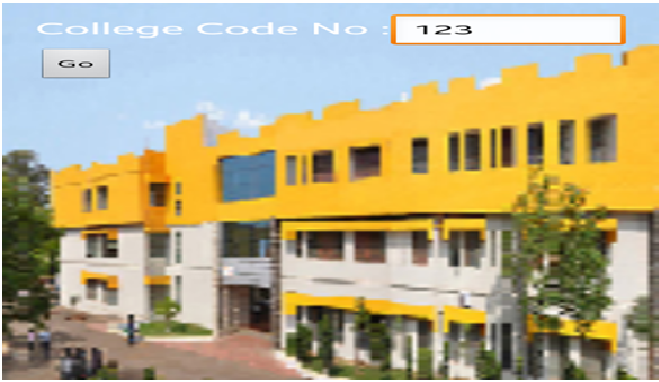
\includegraphics[width=5in]
{AA2}
\caption{College ID Form}
\end{figure}

In this form enter the college code number and click on the go button. When we enter the specific college code then it will go to the specific college and then messege will display like “WELCOME TO SITCollege”. 

\section{Authentication Form}
 \begin{figure}[H]
\centering
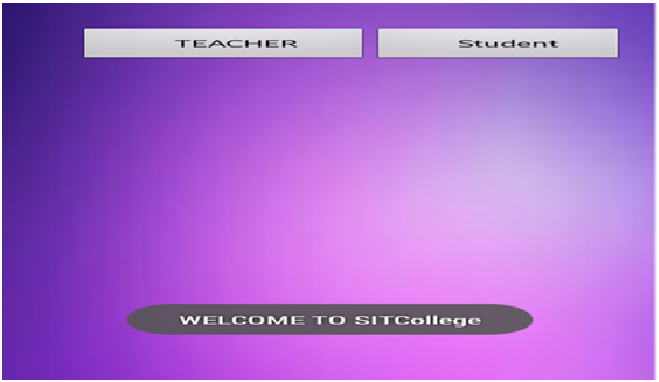
\includegraphics[width=5in]
{AA3}
\caption{Authentication Form}
\end{figure}

This is the authentication form. In this form there are two buttons “Teacher” and “Student”.

 \section{Teacher Login-1}
\begin{figure}[H]
\centering
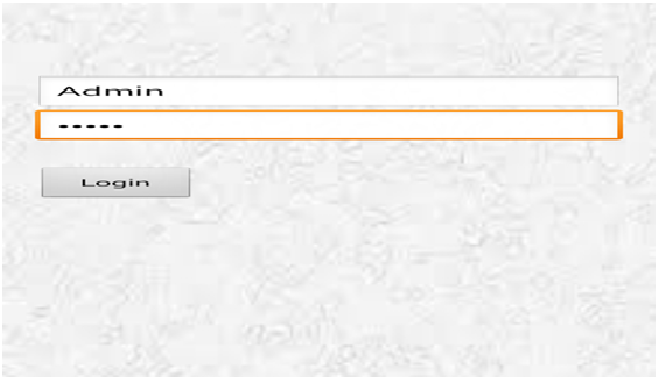
\includegraphics[width=5in]
{AA4}
\caption{Teacher Login-1} 
\end{figure}
This form is open after clicking on “Teacher” button in the Authentication Form. Fill the Name and password and click on the “Login” button. 

\section{Teacher Login-2}
\begin{figure}[H]
\centering
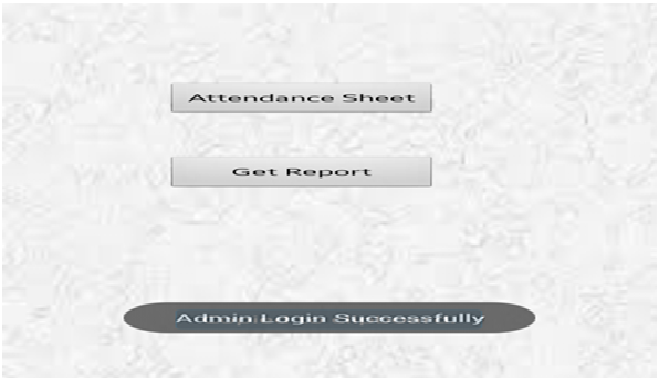
\includegraphics[width=5in]
{AA5}
\caption{Teacher Login-2}
\end{figure}
When teacher filling information in the Teacher Login form then it display message  “Admin  Login Successfully” and it  opens the teacher login-2 form. 

\section{Student Module}
\begin{figure}[H]
\centering
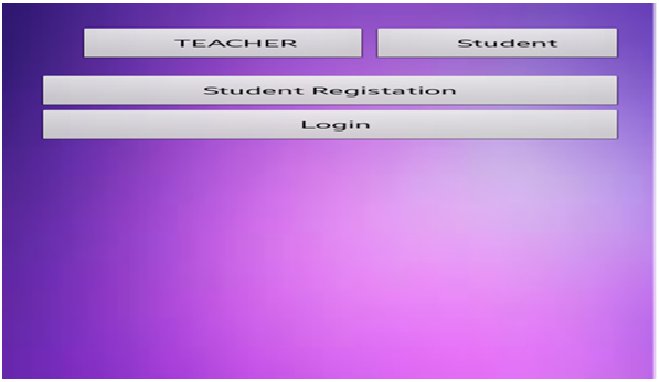
\includegraphics[width=5in]
{AA6}
\caption{Student Module}
\end{figure}

When we click on the “Student” button then this form is open.  There are also two button ”Student Registration ” and the “Login”. 

\section{Student Registration Form}
\begin{figure}[H]
\centering
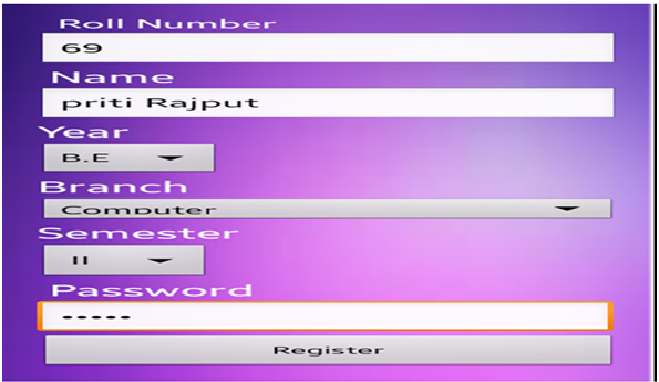
\includegraphics[width=5in]
{AA7}
\caption{Student Registration Form}
\end{figure}

In this form student fill the basic information like Roll Number, Name,  Year, Branch, Semester and Password and then click on the “Register” button.

\section{Student  Login Form}
\begin{figure}[H]
\centering
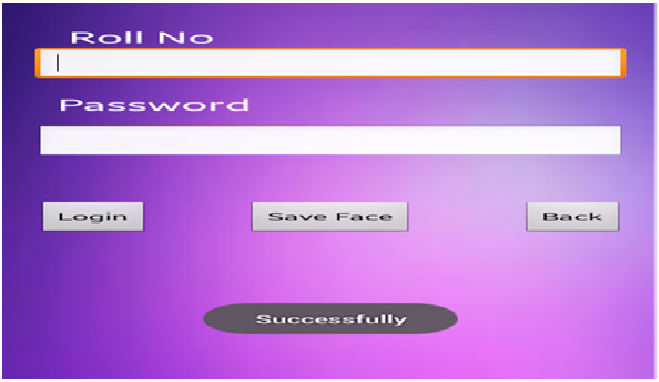
\includegraphics[width=5in]
{AA8}
\caption{Student Login Form.}
\end{figure}

This is the Login form. When Student registration get successfully then Login form is open. 

\section{Student Login Form-1}
\begin{figure}[H]
\centering
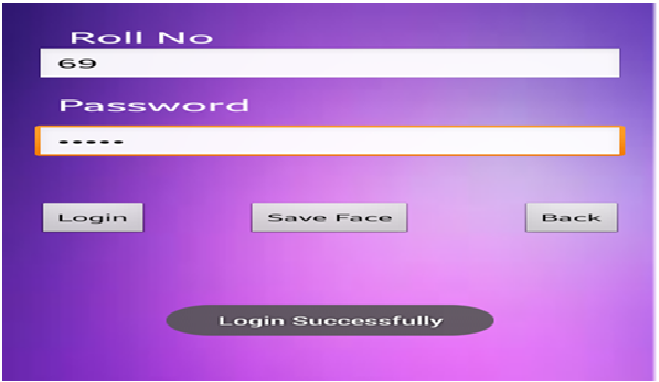
\includegraphics[width=5in]
{AA9}
\caption{Student Login Form-1}
\end{figure}

After filling the information in the Login form then it displays the message “ Login Successfully”. Then click on the “Save Face” button.
 
\section{Face Detection}
\begin{figure}[H]
\centering
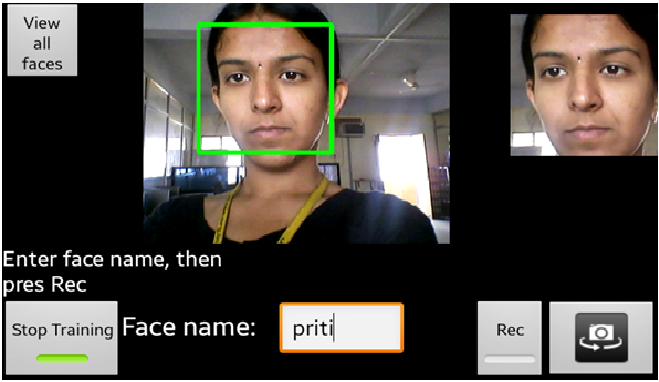
\includegraphics[width=5in]
{AA10}
\caption{Face Detection}
\end{figure}
In this form the student gives his or her face, Name of the face. Then click on the “Rec” button after that click on “Stop Training” button.

\section{Face Recognition-1}
\begin{figure}[H]
\centering
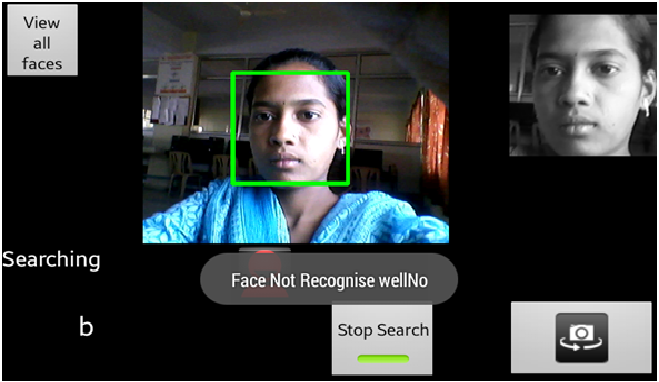
\includegraphics[width=4in]
{AA11}
\caption{Face Recognition-1}
\end{figure}
When the trainee set is completed then it proceeded for the face recognition if the face is not recognized well then it indicate the red and gives the message “Face Not Recognize well No”. 
 
\section{Face Recognition-2}
\begin{figure}[H]
\centering
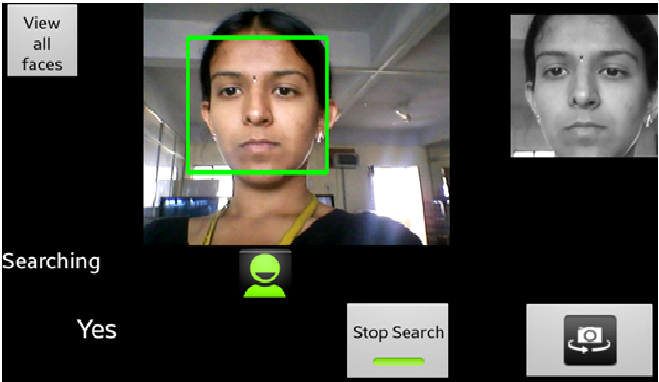
\includegraphics[width=4in]
{AA12}
\caption{Face Recognition-2}
\end{figure}
In this form it searching for the face if the face is matched then it indicated green and then it will go to the Attendance Sheet.

\section{Attendance Sheet}
\begin{figure}[H]
\centering
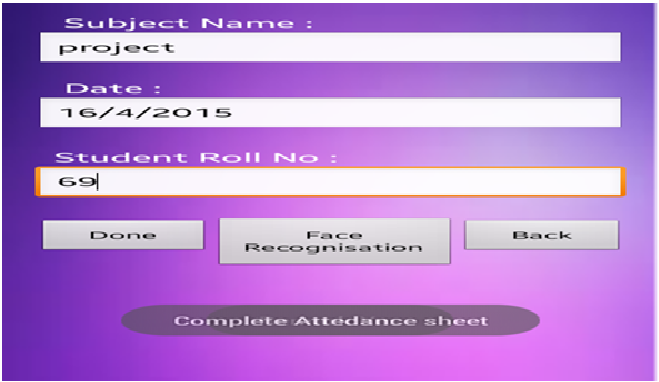
\includegraphics[width=5in]
{AA13}
\caption{Attendance Sheet}
\end{figure}
When the face reorganization is completed then this Attendance Sheet is opened. In this form fill the all field like Subject Name, Date, Student Roll number. After the filling this information click on the “Done” button it gives the message “Complete Attendance Sheet”.

\section{Get Report}
\begin{figure}[H]
\centering
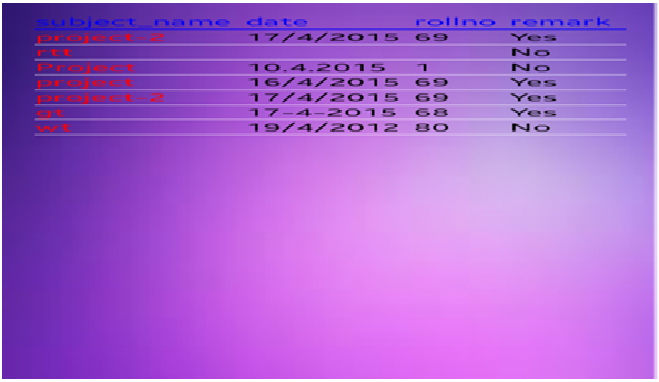
\includegraphics[width=5in]
{AA14}
\caption{Get Report}
\end{figure}
This is “Get Report” form. Here display the report of the registered student. 









